\documentclass[a4paper,twoside]{book}
\usepackage{amd}
\usepackage{fancyvrb}

% %--------------------------------------------------------------------------
% %         General Setting
% %--------------------------------------------------------------------------

\graphicspath{{Images/}{../Images/}} %Path of figures
\setkeys{Gin}{width=0.85\textwidth} %Size of figures
\setlength{\cftbeforechapskip}{3pt} %space between items in toc
\setlength{\parindent}{0.5cm} % Idk
% Theorem System
% The following boxes are provided:
%   Definition:     \defn 
%   Theorem:        \thm 
%   Lemma:          \lem
%   Corollary:      \cor
%   Proposition:    \prop   
%   Claim:          \clm
%   Fact:           \fact
%   Proof:          \pf
%   Example:        \ex
%   Remark:         \rmk (sentence), \rmkb (block)
% Suffix
%   r:              Allow Theorem/Definition to be referenced, e.g. thmr
%   p:              Add a short proof block for Lemma, Corollary, Proposition or Claim, e.g. lemp
%                   For theorems, use \pf for proof blocks

% ======= Real examples : 

% \defn{Definition Name}{
%     A defintion.
% }

% \thmr{Theorem Name}{mybigthm}{
%     A theorem.
% }

% \lem{Lemma Name}{
%     A lemma.
% }

% \fact{
%     A fact.
% }

% \cor{
%     A corollary.
% }

% \prop{
%     A proposition.
% }

% \clmp{}{
%     A claim.
% }{
%     A reference to Theorem~\ref{thm:mybigthm}
% }

% \pf{
%    proof.

% \ex{
%     some examples. 
% }

% \rmk{
%     Some remark.
% }

% \rmkb{
%     Some more remark.
% }

\usepackage{xcolor}

% Define custom colors
\definecolor{defscol}{HTML}{ecd8d7} %For definitions
\definecolor{asumscol}{HTML}{ecd8d7} %For Assumptions

\definecolor{rmkscol}{HTML}{313160} %For remarks
\definecolor{exmscol}{HTML}{e04b52} %For examples

\definecolor{lemscol}{HTML}{2c3943} %For Lemmes
\definecolor{thmscol}{HTML}{595765} %For Theorems
\definecolor{prpscol}{HTML}{9c98b1} %For proposition
\definecolor{corscol}{HTML}{dfd9fd} %For corrolaries

\definecolor{clmscol}{HTML}{165c58} %For claims
\definecolor{facscol}{HTML}{28a8a1} %For facts



% ============================
% Definition
% ============================
\newtcbtheorem[number within=section]{mydefinition}{Definition}
{
    enhanced,
    frame hidden,
    titlerule=0mm,
    toptitle=1mm,
    bottomtitle=1mm,
    fonttitle=\bfseries\large,
    coltitle=black,
    colbacktitle=defscol!40!white,
    colback=defscol!20!white,
}{defn}

\NewDocumentCommand{\defn}{m+m}{
    \begin{mydefinition}{#1}{}
        #2
    \end{mydefinition}
}

\NewDocumentCommand{\defnr}{mm+m}{
    \begin{mydefinition}{#1}{#2}
        #3
    \end{mydefinition}
}

% ============================
% Assumption
% ============================
\newtcbtheorem[use counter from=mydefinition]{myassumption}{Assumption}
{
    enhanced,
    frame hidden,
    titlerule=0mm,
    toptitle=1mm,
    bottomtitle=1mm,
    fonttitle=\bfseries\large,
    coltitle=black,
    colbacktitle=asumscol!40!white,
    colback=asumscol!20!white,
}{asum}

\NewDocumentCommand{\asum}{m+m}{
    \begin{myassumption}{#1}{}
        #2
    \end{myassumption}
}

\NewDocumentCommand{\asumr}{mm+m}{
    \begin{myassumption}{#1}{#2}
        #3
    \end{myassumption}
}

% ============================
% Theorem
% ============================

\newtcbtheorem[use counter from=mydefinition]{mytheorem}{Theorem}
{
    enhanced,
    frame hidden,
    titlerule=0mm,
    toptitle=1mm,
    bottomtitle=1mm,
    fonttitle=\bfseries\large,
    coltitle=black,
    colbacktitle=thmscol!40!white,
    colback=thmscol!20!white,
}{thm}

\NewDocumentCommand{\thm}{m+m}{
    \begin{mytheorem}{#1}{}
        #2
    \end{mytheorem}
}

\NewDocumentCommand{\thmr}{mm+m}{
    \begin{mytheorem}{#1}{#2}
        #3
    \end{mytheorem}
}

\newenvironment{thmpf}{
	{\noindent{\it \textbf{Proof for Theorem.}}}
	\tcolorbox[blanker,breakable,left=5mm,parbox=false,
    before upper={\parindent15pt},
    after skip=10pt,
	borderline west={1mm}{0pt}{thmscol!40!white}]
}{
    \textcolor{thmscol!40!white}{\hbox{}\nobreak\hfill$\blacksquare$} 
    \endtcolorbox
}

\NewDocumentCommand{\thmp}{m+m+m}{
    \begin{mytheorem}{#1}{}
        #2
    \end{mytheorem}

    \begin{thmpf}
        #3
    \end{thmpf}
}

% ============================
% Lemma
% ============================

\newtcbtheorem[use counter from=mydefinition]{mylemma}{Lemma}
{
    enhanced,
    frame hidden,
    titlerule=0mm,
    toptitle=1mm,
    bottomtitle=1mm,
    fonttitle=\bfseries\large,
    coltitle=black,
    colbacktitle=lemscol!40!white,
    colback=lemscol!20!white,
}{lem}

\NewDocumentCommand{\lem}{m+m}{
    \begin{mylemma}{#1}{}
        #2
    \end{mylemma}
}

\newenvironment{lempf}{
	{\noindent{\it \textbf{Proof for Lemma}}}
	\tcolorbox[blanker,breakable,left=5mm,parbox=false,
    before upper={\parindent15pt},
    after skip=10pt,
	borderline west={1mm}{0pt}{lemscol!40!white}]
}{
    \textcolor{lemscol!40!white}{\hbox{}\nobreak\hfill$\blacksquare$} 
    \endtcolorbox
}

\NewDocumentCommand{\lemp}{m+m+m}{
    \begin{mylemma}{#1}{}
        #2
    \end{mylemma}

    \begin{lempf}
        #3
    \end{lempf}
}

% ============================
% Corollary
% ============================

\newtcbtheorem[use counter from=mydefinition]{mycorollary}{Corollary}
{
    enhanced,
    frame hidden,
    titlerule=0mm,
    toptitle=1mm,
    bottomtitle=1mm,
    fonttitle=\bfseries\large,
    coltitle=black,
    colbacktitle=corscol!40!white,
    colback=corscol!20!white,
}{cor}

\NewDocumentCommand{\cor}{+m}{
    \begin{mycorollary}{}{}
        #1
    \end{mycorollary}
}

\newenvironment{corpf}{
	{\noindent{\it \textbf{Proof for Corollary.}}}
	\tcolorbox[blanker,breakable,left=5mm,parbox=false,
    before upper={\parindent15pt},
    after skip=10pt,
	borderline west={1mm}{0pt}{corscol!40!white}]
}{
    \textcolor{corscol!40!white}{\hbox{}\nobreak\hfill$\blacksquare$} 
    \endtcolorbox
}

\NewDocumentCommand{\corp}{m+m+m}{
    \begin{mycorollary}{}{}
        #1
    \end{mycorollary}

    \begin{corpf}
        #2
    \end{corpf}
}

% ============================
% Proposition
% ============================

\newtcbtheorem[use counter from=mydefinition]{myproposition}{Proposition}
{
    enhanced,
    frame hidden,
    titlerule=0mm,
    toptitle=1mm,
    bottomtitle=1mm,
    fonttitle=\bfseries\large,
    coltitle=black,
    colbacktitle=prpscol!30!white,
    colback=prpscol!20!white,
}{prop}

\NewDocumentCommand{\prop}{+m}{
    \begin{myproposition}{}{}
        #1
    \end{myproposition}
}

\newenvironment{proppf}{
	{\noindent{\it \textbf{Proof for Proposition.}}}
	\tcolorbox[blanker,breakable,left=5mm,parbox=false,
    before upper={\parindent15pt},
    after skip=10pt,
	borderline west={1mm}{0pt}{prpscol!40!white}]
}{
    \textcolor{prpscol!40!white}{\hbox{}\nobreak\hfill$\blacksquare$} 
    \endtcolorbox
}



\NewDocumentCommand{\propp}{+m+m}{
    \begin{myproposition}{}{}
        #1
    \end{myproposition}

    \begin{proppf}
        #2
    \end{proppf}
}

% ============================
% Claim
% ============================

\newtcbtheorem[use counter from=mydefinition]{myclaim}{Claim}
{
    enhanced,
    frame hidden,
    titlerule=0mm,
    toptitle=1mm,
    bottomtitle=1mm,
    fonttitle=\bfseries\large,
    coltitle=black,
    colbacktitle=clmscol!40!white,
    colback=clmscol!20!white,
}{clm}

\NewDocumentCommand{\clm}{m+m}{
    \begin{myclaim*}{#1}{}
        #2
    \end{myclaim*}
}

\newenvironment{clmpf}{
	{\noindent{\it \textbf{Proof for Claim.}}}
	\tcolorbox[blanker,breakable,left=5mm,parbox=false,
    before upper={\parindent15pt},
    after skip=10pt,
	borderline west={1mm}{0pt}{clmscol!40!white}]
}{
    \textcolor{clmscol!40!white}{\hbox{}\nobreak\hfill$\blacksquare$} 
    \endtcolorbox
}

\NewDocumentCommand{\clmp}{m+m+m}{
    \begin{myclaim*}{#1}{}
        #2
    \end{myclaim*}

    \begin{clmpf}
        #3
    \end{clmpf}
}

% ============================
% Fact
% ============================

\newtcbtheorem[use counter from=mydefinition]{myfact}{Fact}
{
    enhanced,
    frame hidden,
    titlerule=0mm,
    toptitle=1mm,
    bottomtitle=1mm,
    fonttitle=\bfseries\large,
    coltitle=black,
    colbacktitle=facscol!40!white,
    colback=facscol!20!white,
}{fact}

\NewDocumentCommand{\fact}{+m}{
    \begin{myfact}{}{}
        #1
    \end{myfact}
}

% ============================
% Proof
% ============================

\NewDocumentCommand{\pf}{+m}{
    \begin{proof}
        [\noindent\textbf{Proof.}]
        #1
    \end{proof}
}

% ============================
% Example
% ============================


\newenvironment{myexample}{
    \tcolorbox[blanker,breakable,left=5mm,parbox=false,
    before upper={\parindent15pt},
    after skip=10pt,
	borderline west={1mm}{0pt}{clmscol!40!white}]
}{
    \textcolor{clmscol!40!white}{\hbox{}\nobreak\hfill$\blacksquare$} 
    \endtcolorbox
}

\NewDocumentCommand{\exm}{m+m}{
    \begin{myexample}
	{\noindent{\it \textbf{Example : #1 }}}\\ 
        #2
    \end{myexample}
}


% ============================
% Remark
% ============================


\NewDocumentCommand{\rmk}{+m}{
    {\it \color{rmkscol!40!white}#1}
}

\newenvironment{remark}{
    \par
    \vspace{5pt}
    \begin{minipage}{\textwidth}
        {\par\noindent{\textbf{Remark.}}}
        \tcolorbox[blanker,breakable,left=5mm,
        before skip=10pt,after skip=10pt,
        borderline west={1mm}{0pt}{rmkscol!20!white}]
}{
        \endtcolorbox
    \end{minipage}
    \vspace{5pt}
}

\NewDocumentCommand{\rmkb}{+m}{
    \begin{remark}
        #1
    \end{remark}
}













% % Old styles hh 

% %--------------------------------------------------------------------------
% % 		THEOREMES STYLE
% %--------------------------------------------------------------------------

% %-------		DEFINITION 		-------	
% \newcounter{defo}[chapter]
% \newenvironment{defi}[1]{\refstepcounter{defo} 
% \begin{tcolorbox}[colback=yellow!20!white,colframe=yellow!15!black,title= \textbf{Définition \thechapter \ $\blacklozenge$ \thedefo \ | #1}]}{\end{tcolorbox}}

% %-------		THEOREME 		-------	
% \newcounter{th}[chapter]
% \newenvironment{thm}[1]{\refstepcounter{th}
% \begin{tcolorbox}[colback=mycolor!10,colframe=mycolor!10!black!80,title=\textbf{ Théorème \thechapter \ $\blacklozenge$ \theth \ | #1}]}{\end{tcolorbox}}

% %-------		PROPOSITION 		-------	
% \newcounter{prop}[chapter]
% \newenvironment{propt}[1]{\refstepcounter{prop}
% \begin{tcolorbox}[colback=mycolor!5,colframe=mycolor!10!linkscolor!80 ,title=\textbf{ Proposition \thechapter \ $\blacklozenge$ \theprop \ | #1}]}{\end{tcolorbox}}

% %-------		COROLLAIRE		-------
% \newcounter{cor}[chapter]
% \newenvironment{corr}[1]{\refstepcounter{cor}
% \begin{tcolorbox}[colback=mycolor!2,colframe=mycolor!10!linkscolor!40 ,title= Corolaire \thechapter \ $\blacklozenge$ \thecor \ | #1]}{\end{tcolorbox}}

% %-------		LEMME			-------
% \newcounter{lem}[chapter]
% \newenvironment{lemme}[1]{\refstepcounter{lem}
% \begin{tcolorbox}[colback=mycolor!10!blue!2,colframe=mycolor!50!blue!30,title=\textbf{Lemme \thechapter \ $\blacklozenge$ \thelem \ | #1}]}{\end{tcolorbox}}

% %-------		METHODE 			-------
% \newcounter{met}[chapter]
% \newenvironment{meth}[1]{\refstepcounter{met}
% \begin{tcolorbox}
% [enhanced jigsaw,breakable,pad at break*=1mm,
%  colback=red!20!white,boxrule=0pt,frame hidden,
%  borderline west={1.5mm}{-2mm}{red}] \color{red}
% {\textbf{Méthode \thechapter \ $\blacklozenge$ \themet \ | #1} } \color{black} \\ } {\end{tcolorbox}}

% %-------		REMARQUE 			-------
% \newcommand{\NB}[1]{
% \ \\
% \begin{tabular}{p{0.05\textwidth}p{0.80\textwidth}}
% \hline
% \vspace{-0.1cm} \includegraphics[scale=0.03]{./system/IDEA.png} & 	#1\\
% \hline
% \end{tabular}
% \ 
% \newline \ \newline
%  }

% %-------		EXEMPLE  		-------
% \newenvironment{exm}{ \begin{tcolorbox}
% [enhanced jigsaw,breakable,pad at break*=1mm,
%  colback=cyan!20!white,boxrule=0pt,frame hidden,
%  borderline west={1.5mm}{-2mm}{cyan}] \color{cyan}
% {\textbf{Exemple} } \color{black} \\ } {\end{tcolorbox}}
  % Theorems styles and colors
\usepackage[english]{babel} %Language
\usepackage{framed}

\setlist[itemize]{itemsep=5pt} % Adjust the length as needed
\setlist[enumerate]{itemsep=5pt} % Adjust the length as needed



% \usepackage{lmodern} %  Latin Modern font
% \usepackage{newtxtext,newtxmath}




% %--------------------------------------------------------------------------
% %         General Informations
% %--------------------------------------------------------------------------
\newcommand{\BigTitle}{
    Compilers: Principles, Techniques, \& Tools
    }

\newcommand{\LittleTitle}{
    By Alfred V. Aho et all
    }

    
\begin{document}

% %--------------------------------------------------------------------------
% %         First pages 
% %--------------------------------------------------------------------------
\newgeometry{top=8cm,bottom=.5in,left=2cm,right=2cm}
\subfile{files/0.0.0.titlepage}
\restoregeometry
\thispagestyle{empty}
\setcounter{page}{0}
\tableofcontents
\thispagestyle{empty}
\setcounter{page}{0}

% %--------------------------------------------------------------------------
% %         Core of the document 
% %--------------------------------------------------------------------------
\chapter{Introduction}

The world as we know it depends on programming languages, because all the software running on all the computers was written in some programming language. But, before a program can be run, it first must be translated into a form in which it can be executed by a computer.

The software systems that do this translation are called \textit{compilers}.

\section{Language Processors}

Simply stated, a compiler is a program that can read a program in one language--the \textit{source} language--and translate it into an equivalent program in another language--the \textit{target} language.

An \textit{interpreter} is another common kind of language processor.

The task of collecting the source program is sometimes entrusted to a separate program, called a \textit{preprocessor}.

The compiler may produce an assembly-language program as its output, because assembly language is easier to produce as output and is easier to debug. The assembly language is then processed by a program called an \textit{assembler} that produces relocatable machine code as its output.

The \textit{linker} resolves external memory addresses, where the code in one file may refer to a location in another file. The \textit{loader} then puts together all of the executable object files into memory for execution.

\section{The Structure of a Compiler}

Up to this point we have treated a compiler as a single box that maps a source program into a semantically equivalent target program. If we open up this box a little, we see that there are two parts to this mapping: analysis and synthesis.

The \textit{analysis} part breaks up the source program into constituent pieces and imposes a grammatical structure on them. The analysis part also collects information about the source program and stores it in a data structure called a \textit{symbol table}, which is passed along with the intermediate representation to the synthesis part.

The \textit{synthesis} part constructs the desired target program from the intermediate representation and the information in the symbol table. The analysis part is often called the \textit{front end} of the compiler; the synthesis part is the \textit{back end}.

If we examine the compilation process in more detail, we see that it operates as a sequence of \textit{phases}, each of which transforms one representation of the source program to another.

\subsection{Lexical Analysis}

The first phase of a compiler is called \textit{lexical analysis} or \textit{scanning}. The lexical analyzer reads the stream of characters making up the source program and groups the characters into meaningful sequences called \textit{lexemes}. For each lexeme, the lexical analyzer produces as output a \textit{token} of the form $$\langle\textit{token-name, attribute-value}\rangle$$ that is passes on to the subsequent phase, syntax analysis. In the token, the first component \textit{token-name} is an abstract symbol that is used during syntax analysis, and the second component \textit{attribute-value} points to an entry in the symbol table for this token.

\subsection{Syntax Analysis}

The second phase of the compiler is \textit{syntax analysis} or \textit{parsing}. A typical representation is a \textit{syntax tree} in which each interior node represents an operation and the children of the node represent the arguments of the operation.

\subsection{Semantic Analysis}

The \textit{semantic analyzer} uses the syntax tree and the information in the symbol table to check the source program for semantic consistency with the language definition.

An important part of semantic analysis is \textit{type checking}, where the compiler checks that each operator has matching operands.

The language specification may permit some type conversions called \textit{coercions}.

\subsection{Intermediate Code Generation}

We consider an intermediate form called \textit{three-address code}, which consists of a sequence of assembly-like instructions with three operands per instruction.

\subsection{The Grouping of Phases into Passes}

In an implementation, activities from several phases may be grouped together into a \textit{pass} that reads an input file and writes an output file.

\subsection{Compiler-Construction Tools}

Some commonly used compiler-construction tools include
\begin{enumerate}
    \item \textit{Parser generators} that automatically produce syntax analyzers from a grammatical description of a programming language.
    \item \textit{Scanner generators} that produce lexical analyzers from a regular-expression description of the tokens of a language.
    \item \textit{Syntax-directed translation engines} that produce collections of routines for walking a parse tree and generating intermediate code.
    \item \textit{Code-generator generators} that produce a code generator from a collection of rules for translating each operation of the intermediate language into the machine language for a target machine.
    \item \textit{Data-flow analysis engines} that facilitate the gathering of information about how values are transmitted from one part of a program to each other part.
    \item \textit{Compiler-construction toolkits} that provide an integrated set of routines for construction various phases of a compiler.
\end{enumerate}

\section{The Evolution of Programming Language}
\subsection{The Move to Higher-Level Languages}

One classification is by generation. \textit{First-generation languages} are the machine languages, \textit{second-generation} the assembly languages, and \textit{third-generation} the higher-level languages. \textit{Fourth-generation languages} are languages designed for specific applications. The term \textit{fifth-generation language} has been applied to logic- and constraint-based languages.

Another classification of languages uses the term \textit{imperative} for languages in which a program specifies \textit{how} a computation is to be done and \textit{declarative} for languages in which a program specifies \textit{what} computation is to be done.

The term \textit{von Neumann language} is applied to programming languages whose computational model is based on the von Neumann computer architecture.

An \textit{object-oriented language} is one that supports object-oriented programming, a programming style in which a program consists of a collection of objects that interact with one another.

\textit{Scripting languages} are interpreted languages with high-level operators designed for "gluing together" computations.

\section{Applications of Compiler Technology}
\subsection{implementation of High-Level Programming Languages}

A body of compiler optimizations, known as \textit{data-flow optimizations}, has been developed to analyze the flow of data through the program and removes redundancies across these constructs.

Object-oriented programs are different from those written in many other languages, in that they consist of many more, but smaller, procedures (called \textit{methods} in object-oriented terms).

\subsection{Optimizations for Computer Architectures}

Almost all high-performance systems take advantage of the same two basic techniques: \textit{parallelism} and \textit{memory hierarchies}. Parallelism can be found at several levels: at the \textit{instruction level}, where multiple operations are executed simultaneously and at the \textit{processor level}, where different threads of the same application are run on different processors.

\section{Programming Language Basics}
\subsection{The Static/Dynamic Distinction}

If a language uses a policy that allows the compiler to decide an issue, then we say that the language uses a \textit{static} policy or that the issue can be decided at \textit{compile time}. On the other hand, a policy that only allows a decision to be made when we execute the program is said to be a \textit{dynamic policy} or to require a decision at \textit{run time}.

The \textit{scope} of a declaration of $x$ is the region of the program in which uses of $x$ refer to this declaration. A language uses \textit{static scope} or \textit{lexical scope} if it is possible to determine the scope of a declaration by looking only at the program. Otherwise, the language uses \textit{dynamic scope}.

\subsection{Environments and States}

\begin{figure}[htbp]
    \centering
    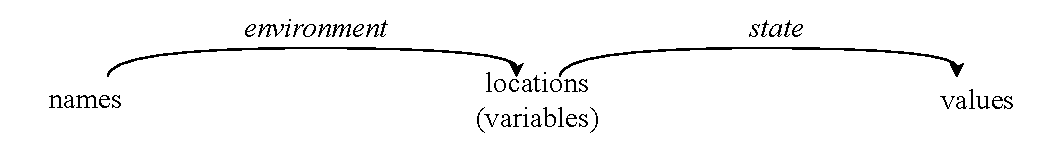
\includegraphics[width=\linewidth]{Figure1 8.pdf}
    \caption{Two-stage mapping from names to values}
    \label{figure:1.8}
\end{figure}

The association of names with locations in memory (the \textit{store}) and then with values can be described by two mappings that change as the program runs:
\begin{enumerate}
    \item The \textit{environment} is a mapping from names to locations in the store.
    \item The \textit{state} is a mapping from locations in store to their values.
\end{enumerate}

The environment and state mappings in Fig.\;\ref{figure:1.8} are dynamic, but there are a few exceptions:
\begin{enumerate}
    \item \textit{Static versus dynamic binding} of names to locations.
    \item \textit{Static versus dynamic binding} of locations to values.
\end{enumerate}

\begin{framed}
\begin{center}
    \textbf{{\large Names, Identifiers, and Variables}}
\end{center}

An \textit{identifier} is a string of characters, typically letters or digits, that refers to (identifies) an entity. Composite names are called \textit{qualified} names.

A \textit{variable} refers to a particular location of the store.
\end{framed}

\subsection{Static Scope and Block Structure}
\label{section:1.6.3}

The scope rules for C are based on program structure; the scope of a declaration is determined implicitly by where the declaration appears in the program. Later languages also provide explicit control over scopes through the use of keywords like \textbf{public}, \textbf{private} and \textbf{protected}.

A \textit{block} is a grouping of declarations and statements. C uses braces \texttt{\{} and \texttt{\}} to delimit a block; the alternative use of \textbf{begin} and \textbf{end} for the same purpose dates back to Algol.

In C, the syntax of blocks is given by
\begin{enumerate}
    \item One type of statement is a block. Blocks can appear anywhere that other types of statement can appear.
    \item A block is a sequence of declarations followed by a sequence of statements, all surrounded by braces.
\end{enumerate}

Note that this syntax allows blocks to be nested inside each other. This nesting property is referred to as \textit{block structure}.

\subsection{Explicit Access Control}

Through the use of keywords like \textbf{public}, \textbf{private}, and \textbf{protected}, object-oriented languages provide explicit control over access to member names in a superclass. These keywords support \textit{encapsulation} by restricting access.

\subsection{Dynamic Scope}

Technically, any scoping policy is dynamic if it is based on factor(s) that can be known only when the program executes. The term \textit{dynamic scope}, however, usually refers to the following policy: a use of a name $x$ refers to the declaration of $x$ in the most recently called procedure with such a declaration.

\begin{framed}
    \begin{center}
        \textbf{{\large Declarations and Definitions}}
    \end{center}

    In C++, a method is declared in a class definition, by giving the types of the arguments and result of the method (often called the \textit{signature} for the method).
\end{framed}

\subsection{Parameter Passing Mechanisms}

\textit{Actual parameters} (the parameters used in the call of a procedure) are associated with the \textit{formal parameters} (those used in the procedure definition).

\subsubsection{Call-by-Value}

In \textit{call-by-value}, the actual parameter is evaluated (if it is an expression) or copied (if it is a variable).

\subsubsection{Call-by-Reference}

In \textit{call-by-reference}, the address of the actual parameter is passed to the callee as the value of the corresponding formal parameter.

\subsection{Aliasing}

It is possible that two formal parameters can refer to the same location; such variables are said to be \textit{aliases} of one another.

\chapter{A Simple Syntax-Directed Translator}
\section{Introduction} 

The \textit{syntax} of a programming language defines what its programs, while the \textit{semantics} of the language defines what its program mean; that is, what each program does when it executes.

A lexical analyzer allows a translator to handle mutlicharacter constructs like identifiers, which are written as sequences of charactersm, but are treated as units called \textit{tokens} during syntax analysis.

\begin{figure}[htbp]
    \centering
    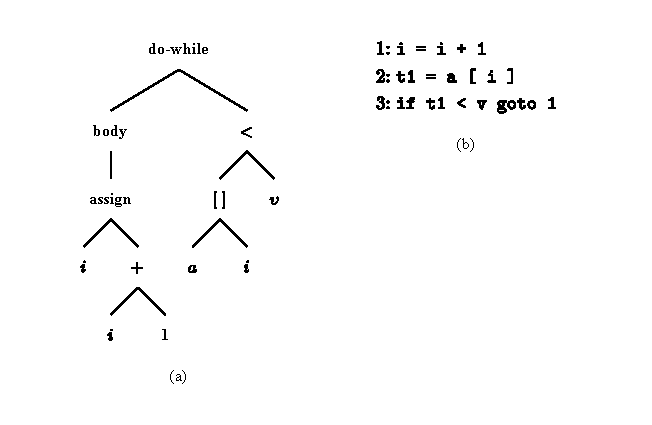
\includegraphics[width=\linewidth]{Figure2 4.pdf}
    \caption{Intermediate code for "\texttt{do i=i+1; while(a[i]<v);}"}
    \label{figure:2.4}
\end{figure}

Two forms of intermediate code are illustrated in Fig.\;\ref{figure:2.4}. One form, called \textit{abstract syntax trees} or simply \textit{syntax trees}, represents the hierarchical systematic structure of the source program.

\section{Syntax Definition}

A grammar naturally describes the hierarchical structure of most programming language constructs. For example, an if-else statement in Java can have the form
\begin{center}
    \textbf{if} (expression) statement \textbf{else} statement
\end{center}

Using the variable \textit{expr} to denote an expression and the variable \textit{stmt} to denote a statement, this structuring rule can be expressed as
\begin{center}
    \textit{stmt} $\rightarrow$ \textbf{if} (\textit{expr}) \textit{stmt} \textbf{else} \textit{stmt}
\end{center}
in which the arrow may be read as "can have the form." Such a rule is called a \textit{production}. In a production, lexical elements are called \textit{terminals}. Variables like \textit{expr} and \textit{stmt} represent sequences of terminals and are called \textit{nonterminals}.

\subsection{Definition of Grammars}

A \textit{context-free grammar} has four components:
\begin{enumerate}
    \item A set of \textit{terminal} symbols, sometimes referred to as "tokens."
    \item A set of \textit{nonterminals}, sometimes called "syntactic variables."
    \item A set of \textit{productions}, where each production consists of a nonterminal, called the \textit{head} or \textit{left side} of the production, an arrow, and a sequence of terminals and/or nonterminals, called the \textit{body} or \textit{right side} of the production.
    \item A designation of one of the nonterminals as the \textit{start} symbol.
\end{enumerate}

\begin{framed}
    \begin{center}
        \textbf{{\large Tokens Versus Terminals}}
    \end{center}

    A token consists of two components, a token name and an attribute value. The token names are abstract symbols that are used by the parser for syntax analysis. Often, we shall call these token names \textit{terminals}, since they appear as terminal symbols in the grammar for a programming language.
\end{framed}

We say a production is \textit{for} a nonterminal if the nonterminal is the head of the production. The string of zero terminals, written as $\epsilon$, is called the \textit{empty} string.

\subsection{Derivations}

The terminal strings that can be derived from the start symbol form the \textit{language} defined by the grammar.

\textit{Parsing} is the problem of taking a string of terminals and figuring out how to derive it from the start symbol of the grammar, and if it cannot be derived from the start symbol of the grammar, then reporting syntax errors within the string.

\subsection{Parse Trees}

A parse tree pictorially shows how the start symbol of a grammar derives a string in the language.

Formally, given a context-free grammar, a \textit{parse tree} according to the grammar is a tree with the following properties:
\begin{enumerate}
    \item The root is labeled by the start symbol.
    \item Each leaf is labeled by a terminal or by $\epsilon$.
    \item Each interior node is labeled by a nonterminal.
    \item If $A$ is the nonterminal labeling some interior node and $X_1,X_2,\cdots,X_n$ are the labels of the children of that node from left to right, then there must be a production $A\rightarrow X_1X_2\cdots X_n$.
\end{enumerate}

\begin{framed}
    \begin{center}
        \textbf{{\large Tree Terminology}}
    \end{center}

    Tree data structures figure prominently in compiling.
    \begin{itemize}
        \item A tree consists of one or more \textit{nodes}. Nodes may have \textit{labels}.
        \item Exactly one node is the \textit{root}. All nodes except the root have a unique \textit{parent}; the root has no parent.
        \item If node $N$ is the parent of node $M$, then $M$ is a \textit{child} of $N$. The children of one node are called \textit{siblings}. They have an order, \textit{from the left}, and when we draw trees, we order the children 
        \item A node with no children is called a \textit{leaf}. Other nodes -- those with one or more children -- are \textit{interior nodes}.
        \item A \textit{descendant} of a node $N$ is either $N$ itself, a child of $N$, a child of a child of $N$, and so on, for any number of levels. We say node $N$ is an \textit{ancestor} of node $M$ if $M$ is a descendant of $N$.
    \end{itemize}
\end{framed}

From left to right, the leaves of a parse tree form the \textit{yield} of the tree, which is the string \textit{generated} or \textit{derived} from the nonterminal at the root of the parse tree.

The process of finding a parse tree for a given string of terminals is called \textit{parsing} that string.

\subsection{Ambiguity}

We have to be careful in talking about \textit{the} structure of a string according to a grammar. A grammar can have more than one parse tree generating a given string of terminals. Such a grammar is said to be \textit{ambiguous}.

\subsection{Associativity of Operators}

We say that the operator $+$ \textit{associates} to the left, because an operand with plus signs on both sides of it belongs to the operator to its left.

\subsection{Precedence of Operators}

We say that $*$ has \textit{higher precedence} than $+$ if $*$ takes its operands before $+$ does.

\section{Syntax-Directed Translation}

This section introduces two concepts related to syntax-directed translation:
\begin{itemize}
    \item\textit{Attributes}. An \textit{attribute} is any quantity associated with a programming construct.
    \item(\textit{Syntax-directed}) \textit{translation schemes}. A \textit{translation scheme} is a notation for attaching program fragments to the productions of a grammar.
\end{itemize}

\subsection{Postfix Notation}

The \textit{postfix notation} for an expression $E$ can be defined inductively as follows:
\begin{enumerate}
    \item If $E$ is a variable or constant, then the postfix notation for $E$ is $E$ itself.
    \item If $E$ is an expression of the form $E_1$ \textbf{op} $E_2$, where \textbf{op} is any binary operator, then the postfix notation for $E$ is $E_1'$ $E_2'$ \textbf{op}, where $E_1'$ and $E_2'$ are the postfix notations for $E_1$ and $E_2$, respectively.
    \item If $E$ is a parenthesized expression of the form $(E_1)$, then the postfix notation for $E$ is the same as the postfix notation for $E_1$.
\end{enumerate}

No parentheses are needed in postfix notation, because the position and \textit{arity} (number of arguments) of the operators permits only one decoding of a postfix expression.

\subsection{Synthesized Attributes}

A \textit{syntax-directed definition} associates:
\begin{enumerate}
    \item With each grammar symbol, a set of attributes, and
    \item With each production, a set of \textit{semantic rules} for computing the values of the attributes associated with the symbols appearing in the production.
\end{enumerate}

A parse tree showing the attribute values at each node is called an \textit{annotated} parse tree.

An attribute is said to be \textit{synthesized} if its value at a parse-tree node $N$ is determined from attribute values at the children of $N$ and at $N$ itself.

\subsection{Tree Traversals}

A \textit{traversal} of a tree starts at the root and visits each node of the tree in some order.

A \textit{depth-first} traversal starts at the root and recursively visits the children of each node in any order, not necessarily from left to right.

Synthesized attributes can be evaluated during any \textit{bottom-up} traversal, that is, a traversal that evaluates attributes at a node after having evaluated attributes at its children.

\subsection{Translation Schemes}

\begin{framed}
    \begin{center}
        \textbf{{\large Preorder and Postorder Traversals}}
    \end{center}

    Often, we traverse a tree to perform some particular action at each node. If the action is done when we first visit a node, then we may refer to the traversal as a \textit{preorder traversal}. Similarly, if the action is done just before we leave a node for the last time, then we say it is a \textit{postorder traversal} of the tree.

    The \textit{preorder} of a (sub)tree rooted at node $N$ consists of $N$, followed by the preorders of the subtrees of each of its children, if any, from the left. The \textit{postorder} of a (sub)tree rooted at $N$ consists of the postorders of each of the subtrees for the children of $N$, if any, from the left, followed by $N$ itself.
\end{framed}

Program fragments embedded within production bodies are called \textit{semantic actions}.

\section{Parsing}

Most parsing methods fall into one of two classes, called the \textit{top-down} and \textit{bottom-up} methods.

\subsection{Top-Down Parsing}

The current terminal being scanned in the input is frequently referred to as the \textit{lookahead} symbol.

\subsection{Predictive Parsing}

\textit{Recursive-descent parsing} is a top-down method of syntax analysis in which a set of recursive procedures is used to process the input. Here, we consider a simple form of recursive-descent parsing, called \textit{predictive parsing}, in which the lookahead symbol unambiguously determines the flow of control through the procedure body for each nonterminal.

\subsection{Designing a Predictive Parser}

Recall that a \textit{predictive parser} is a program consisting of a procedure for every nonterminal.

\subsection{Left Recursion}

Consider a nonterminal $A$ with tow productions $$A\;\rightarrow\;A\alpha\;|\;\beta$$ where $\alpha$ and $\beta$ are sequences of terminals and nonterminals that do not start with $A$.

The nonterminal $A$ and its production are said to be \textit{left recursive}, because the production $A\to A\alpha$ has $A$ itself as the leftmost symbol on the right side.

The same effect can be achieved by rewriting the productions for $A$ in the following manner, using a new nonterminal $R$:
\begin{align*}
    &A\;\to\;\beta R\\
    &R\;\to\;\alpha R\;|\;\epsilon
\end{align*}

Nonterminal $R$ and its production $R\to\alpha R$ are \textit{right recursive} because this production for $R$ has $R$ itself as the last symbol on the right side.

\section{A Translator for Simple Expressions}

\subsection{Abstract and Concrete Syntax}

In an \textit{abstract syntax tree} for an expression, each interior node represents an operator; the children of the node represent the operands of the operator.

Abstract syntax trees, or simply \textit{syntax trees}, resemble parse trees to an extent. Many nonterminals of a grammar represent programming constructs, but others are "helpers" of one sort of another. In the syntax tree, these helpers typically are not needed and are hence droped. To emphasize the contrast, a parse tree is sometimes called a \textit{concrete syntax tree}, and the underlying grammar is called a \textit{concrete syntax} for the language.

\begin{figure}[htbp]
    \centering
    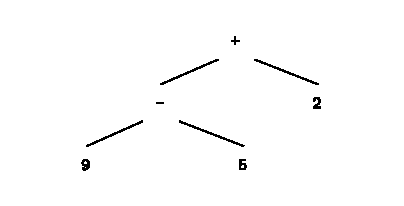
\includegraphics[width=\linewidth]{Figure2 22.pdf}
    \caption{Syntax tree for \texttt{9-5+2}}
    \label{Figure:2.22}
\end{figure}

In the syntax tree in Fig.\;\ref{Figure:2.22}, each interior node is associated with an operator, with no "helper" nodes for \textit{single productions} (a production whose body consists of a single nonterminal, and nothing else) or for $\epsilon$-productions.

\subsection{Simplifying the Translator}

When the last statement executed in a procedure body is a recursive call to the same procedure, the call is said to be \textit{tail recursive}.

\subsection{The Complete Program}

\begin{Verbatim}
    import java.io.*
    class Parser {
        static int lookahead;

        public Parser() throws IOException {
            lookahead = System.in.read();
        }

        void expr() throws IOException {
            term();
            while(true) {
                if (lookahead == '+') {
                    match('+'); term(); System.out.write('+');
                }
                else if (lookahead == '-') {
                    match('-'); term(); System.out.write('-');
                }
                else return;
            }
        }

        void term() throws IOException {
            if (Character.isDigit((char)lookahead)) {
                System.out.write((char)lookahead); match(lookahead);
            }
            else throw new Error("syntax error");
        }
    }

    public class Postfix {
        public static void main(String[] args) throws IOException {
            Parser parse = new Parser();
            parse.expr(); System.out.write('\n');
        }
    }
\end{Verbatim}
\begin{figure}[htbp]
    \caption{Java program to translate infix expressions into postfix form}
    \label{Figure:2.27}
\end{figure}

The function \texttt{Parser}, with the same name as its class, is a \textit{constructor}; it is called automatically when an object of the class is created.

The construction \texttt{(char)lookahead} \textit{casts} or coerces \texttt{lookahead} to be a character.

\section{Lexical Analysis}

A sequence of input characters that comprises a single token is called a \textit{lexeme}.

\subsection{Recognizing Keywords and Identifiers}

Most languages use fixed character strings as punctuation marks or to identify consturcts. Such character strings are called \textit{keywords}.

Grammars routinely treat identifiers as terminals to simplify the parser, which can then expect the same terminal, say \textbf{id}, each time any identifier appears in the input. For example, on input
\begin{equation}
    \texttt{count = count + increment;}
\end{equation}
the parser works with the terminal stream \textbf{id}\texttt{=}\textbf{id}\texttt{+}\textbf{id}.

Keywords generally satisfy the rules for forming identifiers, so a mechanism is needed f deciding when a lexeme forms a keyword and when it forms an identifier. The problem is easier to resolve if keywords are \textit{reserved}; i.e., if they cannot be used as identifiers.

The lexical analyzer in this section solves two problems by using a table to hold character strings:
\begin{itemize}
    \item\textit{Single Representation.}
    \item\textit{Reserved Words}.
\end{itemize}

In Java, a string table can be implemented as a hash table using a class called \textit{Hashtable}.

\section{Symbol Tables}

\textit{Symbol tables} are data structures that are used by compilers to hold information about source-program constructs.

A program consists of blocks with optional declarations and "statements" consisting of single identifiers. Each such statement represents a use of the identifier. Here is a sample program in this language:
\begin{equation}
    \texttt{\{ int x; char y; \{ bool y; x; y; \} x; y; \}}
    \label{2.7}
\end{equation}

\subsection{Symbol Table Per Scope}

The term \textit{scope} by itself refers to a portion of a program that is the scope of one or more declarations.

The \textit{most-closely nested} rule for blocks is that an identifier $x$ is in the scope of the most-closely nested declaration of $x$; that is, the declaration of $x$ found by examining blocks inside-out, starting with the block in which $x$ appears.

\section{Intermediate Code Generation}
\subsection{Two Kinds of Intermediate Representations}

In addition to creating an intermediate representation, a compiler front end checks that the source program follows the syntactic and semantic rules of the source language. This checking is called \textit{static checking}; in general "static" means "done by  the compiler."

\subsection{Construction of Syntax Trees}
\subsubsection{Syntax Trees for Expressions}

The table in Fig.\;\ref{Figure:2.41}  specifies the correspondence between the concrete and abstract syntax for several of the operators of Java.

The subscript \textit{unary} in $\texttt{-}_{unary}$ is solely to distinguish a leading unary minus sign from a binary minus sign.

\begin{equation*}
    \begin{array}{cc}\text{Concrete Syntax}&\text{Abstract Syntax}\\\texttt{=} &\textbf{assign}\\\texttt{||} &\textbf{cond}\\\texttt{\&\&}&\textbf{cond}\\\texttt{== !=}&\textbf{rel}\\\texttt{< <= >= >}&\textbf{rel}\\\texttt{+ -}&\textbf{op}\\\texttt{* / \%}&\textbf{op}\\\texttt{!}&\textbf{not}\\\texttt{-}_{unary}&\textbf{minus}\\\texttt{[]}&\textbf{access}\end{array}
\end{equation*}
\begin{figure}[htbp]
    \caption{Concrete and abstract syntax for several Java operators}
    \label{Figure:2.41}
\end{figure}

\subsection{Static Checking}

Static checking includes:
\begin{itemize}
    \item\textit{Syntactic Checking}.
    \item\textit{Type Checking}.
\end{itemize}

\subsubsection{L-values and R-values}

The terms \textit{l-value} and \textit{r-value} refer to values that are appropriate on the left and right sides of an assignment, respectively.

\subsubsection{Type Checking}

Type checking assures that the type of a construct matches that expected by its context.

The idea of matching actual with expected types continues to apply, even in the following situations:
\begin{itemize}
    \item\textit{Coercions}. A \textit{coercion} occurs if the type of an operand is automatically converted to the type expected by the operator.
    \item\textit{Overloading}. A symbol is said to be \textit{overloaded} if it has different meanings depending on its context.
\end{itemize}

\subsection{Three-Address Code}
\subsubsection{Better Code for Expressions}

We can avoid some copy instructions by modifying the translation functions to generate a partial instruction that computes, say \texttt{j+k}, but does not commit to where the result is to be placed, signified by \textbf{null} address for the result:
\begin{equation}
    \textbf{null}\texttt{ = j + k}
\end{equation}

\chapter{Lexical Analysis}

To implement a lexical analyzer by hand, it helps to start with a diagram or other description for the lexemes of each token. We can then write code to identify each occurrence of each lexeme on the input and to return information about the token identified.

We can also produce a lexical analyzer automatically by specifying the lexeme patterns to a \textit{lexical-analysis generator} and compiling those patterns into code that functions as a lexical analyzer.

\section{The Role of the Lexical Analyzer}

Since the lexical analyzer is the part of the compiler that reads the source text, it may perform certain other tasks besides identification of lexemes. One such task is stripping out comments and \textit{whitespace} (blank, newline, tab, and perhaps other characters that are used to separate tokens in the input).

Sometimes, lexical analyzers are divided into a cascade of two processes:
\begin{itemize}
    \item[a)]\textit{Scanning} consists of the simple processes that do not require tokenization of the input.
    \item[b)]\textit{Lexical analysis} proper is the more complex portion, where the scanner produces the sequence of tokens as output.
\end{itemize}

\subsection{Tokens, Patterns, and Lexemes}

When discussing lexical analysis, we use three related but distinct terms:
\begin{itemize}
    \item A \textit{token} is a pair consisting of a token name and an optional attribute value.
    \item A \textit{pattern} is a description of the form that the lexemes of a token may take. In the case of a keyword as a token, the pattern is just the sequence of characters that form the keyword. For identifiers and some other tokens, the pattern is a more complex structure that is \textit{matched} by many strings.
    \item A \textit{lexeme}  is a sequence of characters in the source program that matches the pattern for a token and is identified by the lexical analyzer as an instance of that token.
\end{itemize}

\section{Input Buffering}

% %--------------------------------------------------------------------------
% %         Bibliographie 
% %--------------------------------------------------------------------------
\end{document}